% DO NOT COMPILE THIS FILE DIRECTLY!
% This is included by the other .tex files.

\begin{frame}[t,plain]
  \titlepage
\end{frame}

%---------------------------------------------------------------------
\section{Problem Overview \& Motivation}

%\begin{frame}[t]{MagLIF}
%  8 minutes
%  \begin{itemize}
%    \item What is MagLIF?
%    \item How does it work?
%    \item What makes it interesting to us?
%    \item What can you draw from Literature?
%    \item Where is our Investigation?
%    \item What are still issues that they have with MagLIF? (See Tech-X talk)
%    \item How does what we do "Kinetic Closures" help with the fluid model
%  \end{itemize}
%
%\end{frame}
\begin{frame}[t, label=current]{Direct Drive - 1}
 \begin{figure}[!htbp]
   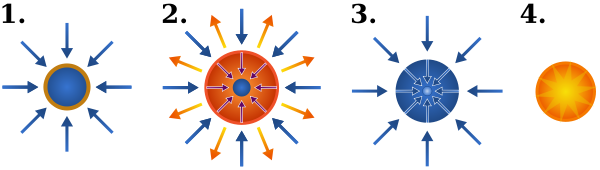
\includegraphics[width=0.8\linewidth]{fig/600pxICF.png}
   \centering
 \end{figure}
 \footnote{Inertial Confinement Fusion Wiki}
\end{frame}


\begin{frame}[t, label=current]{Direct Drive/RT}
  \minipage{\textwidth}
  \minipage{0.57\textwidth}
  \begin{figure}[!htbp]
   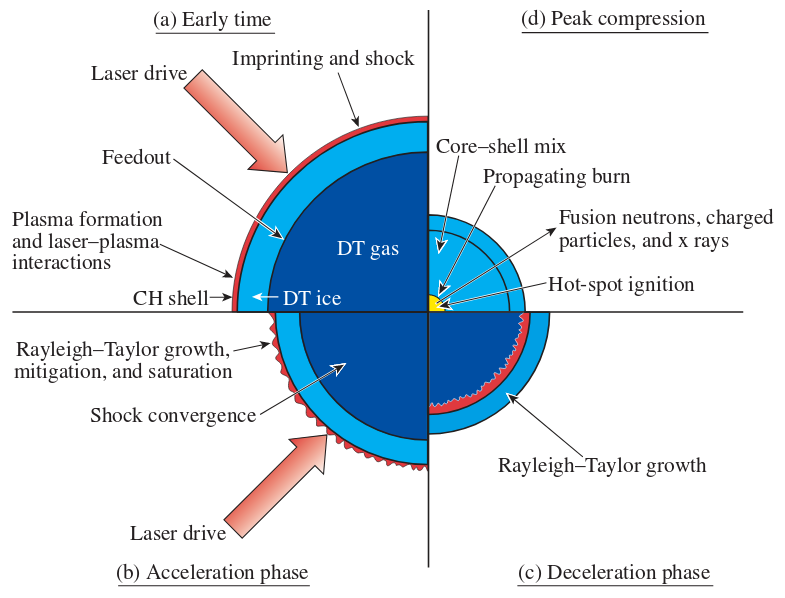
\includegraphics[width=1.0\linewidth]{../fig/DDfusion}
   \centering
  \end{figure}

  \endminipage\hfill
  \minipage{0.42\textwidth}
  \begin{itemize}
    \item Heavy fluid 
    \item Light fluid
    \item Gravity 
    \item Stabilizing Magnetic fields
  \end{itemize}

  \endminipage\hfill
  \endminipage


  \vspace{-0.5cm}

 \footnote{\cite{craxton2015}}


\end{frame}


\section{Previous Equation System \& Modeling Capabilities}

\begin{frame}[t]{Eqn System $-$ 1 PreExisting FVM code}
  \minipage{\textwidth}
  \minipage{0.42\textwidth}
  \begin{align*}
    \pfrac{\rho}{t} + \nabla \cdot \left[\rho \mathbf{u}\right] &= 0 \\
    \pfrac{\rho \mathbf{u}}{t} + \nabla \cdot \left[\rho \mathbf{u}\mathbf{u}^T + \mathbb{I}P\right] = 0 \\
    \pfrac{\epsilon}{t} + \nabla \cdot \left[\left(\epsilon + P \right)\mathbf{u}\right] &= 0 \\
    \epsilon = \epsilon_{internal} + \frac{1}{2}\rho|\mathbf{u}|^2 &\\
    P = \rho \epsilon_{internal} (\gamma - 1) &
  \end{align*}
  \endminipage\hfill
  \minipage{0.57\textwidth}
 \begin{figure}[!htbp]
   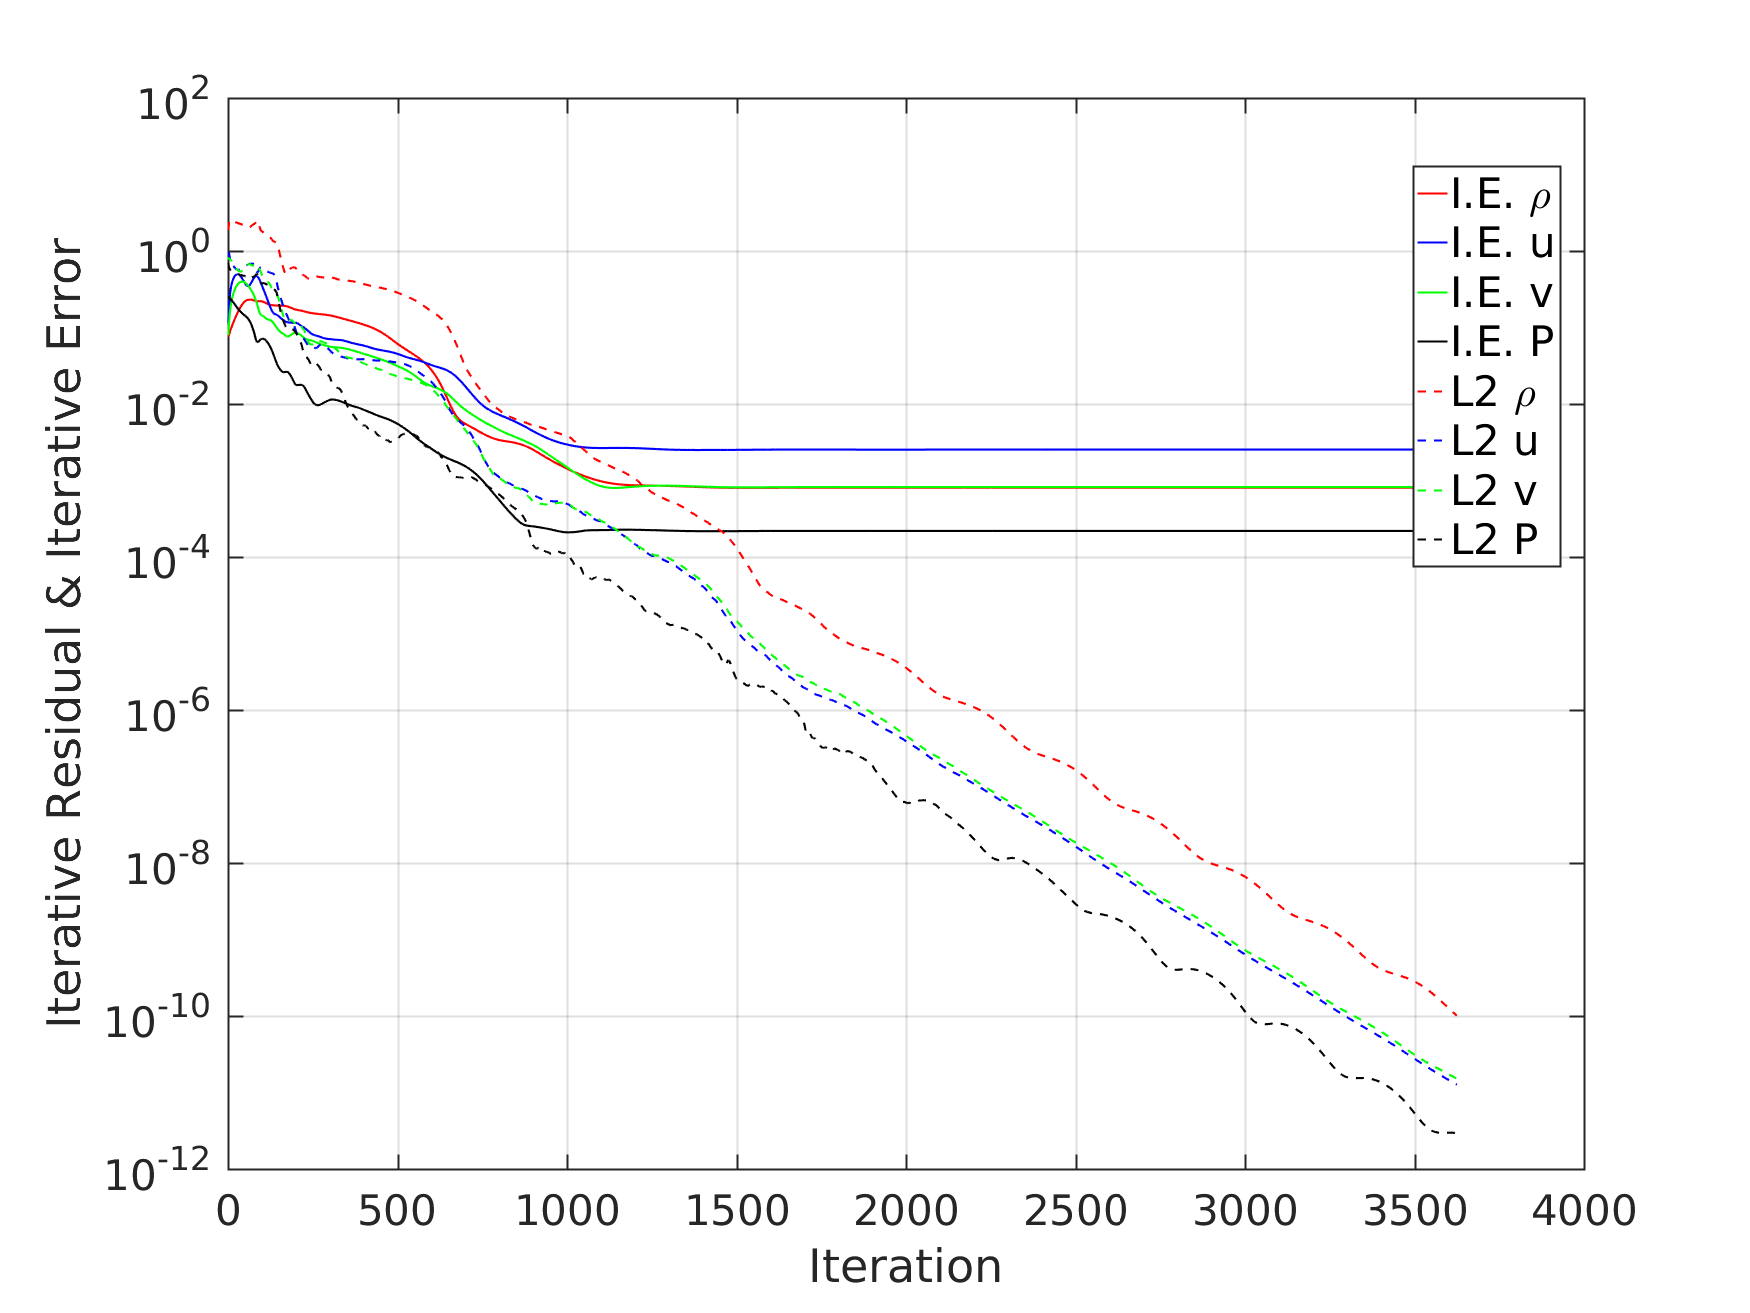
\includegraphics[width=1.0\linewidth]{fig/Iter_SB}
   \centering
 \end{figure}

  \endminipage\hfill
  \endminipage

\end{frame}

\begin{frame}[t]{Eqn System $-$ 2 PreExisting FVM code}
  \minipage{\textwidth}
  \minipage{0.48\textwidth}
  \begin{figure}[!htbp]
    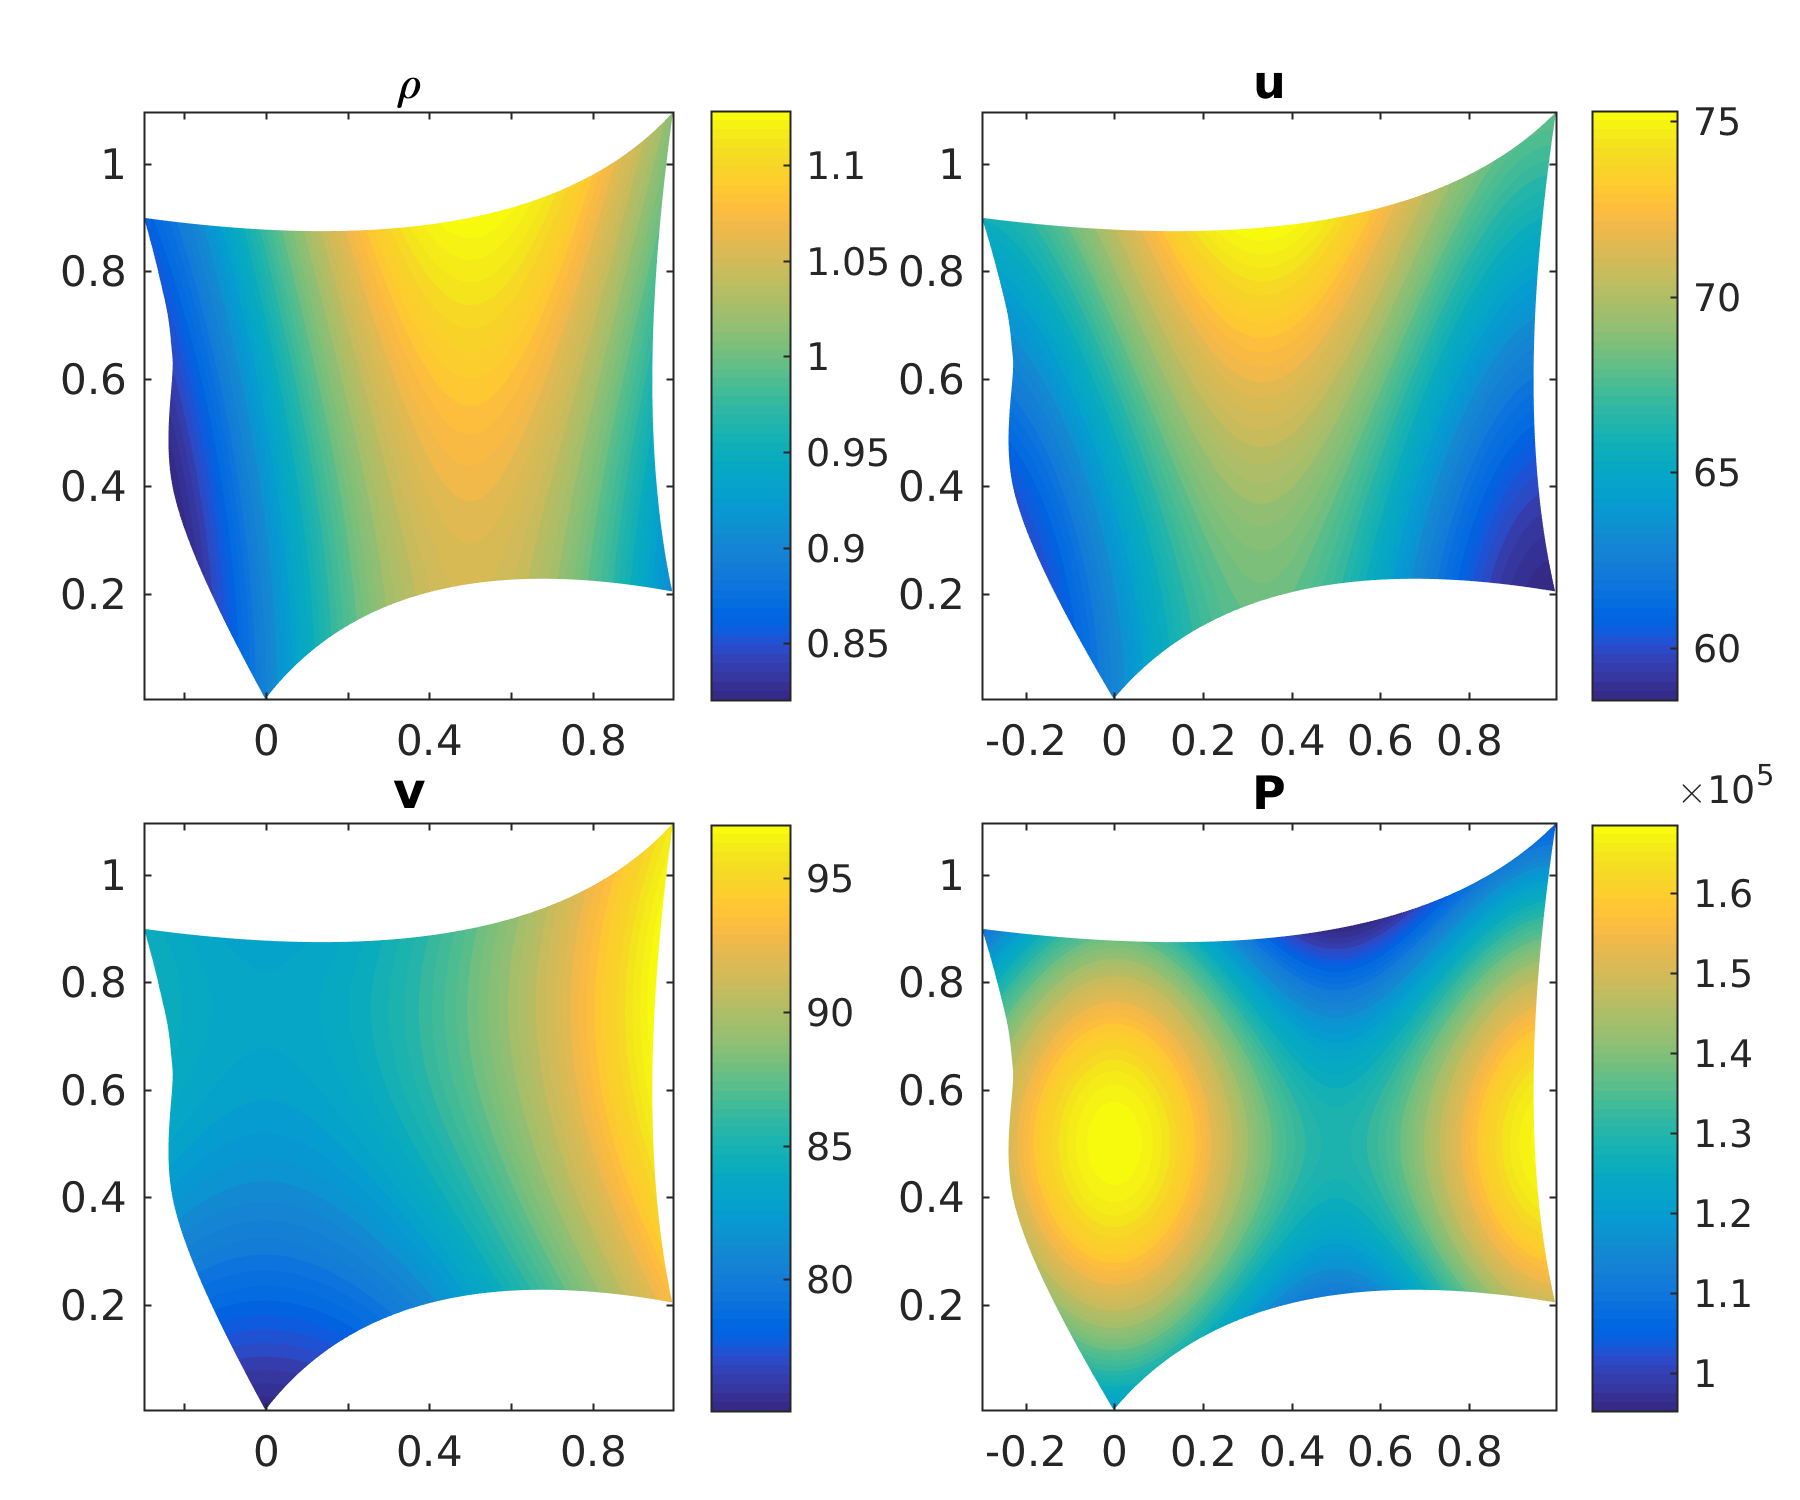
\includegraphics[width=1.0\linewidth]{fig/MMS_mesh6_SB_soln}
    \centering
  \end{figure}
  \endminipage\hfill
  \minipage{0.48\textwidth}
  \begin{figure}[!htbp]
    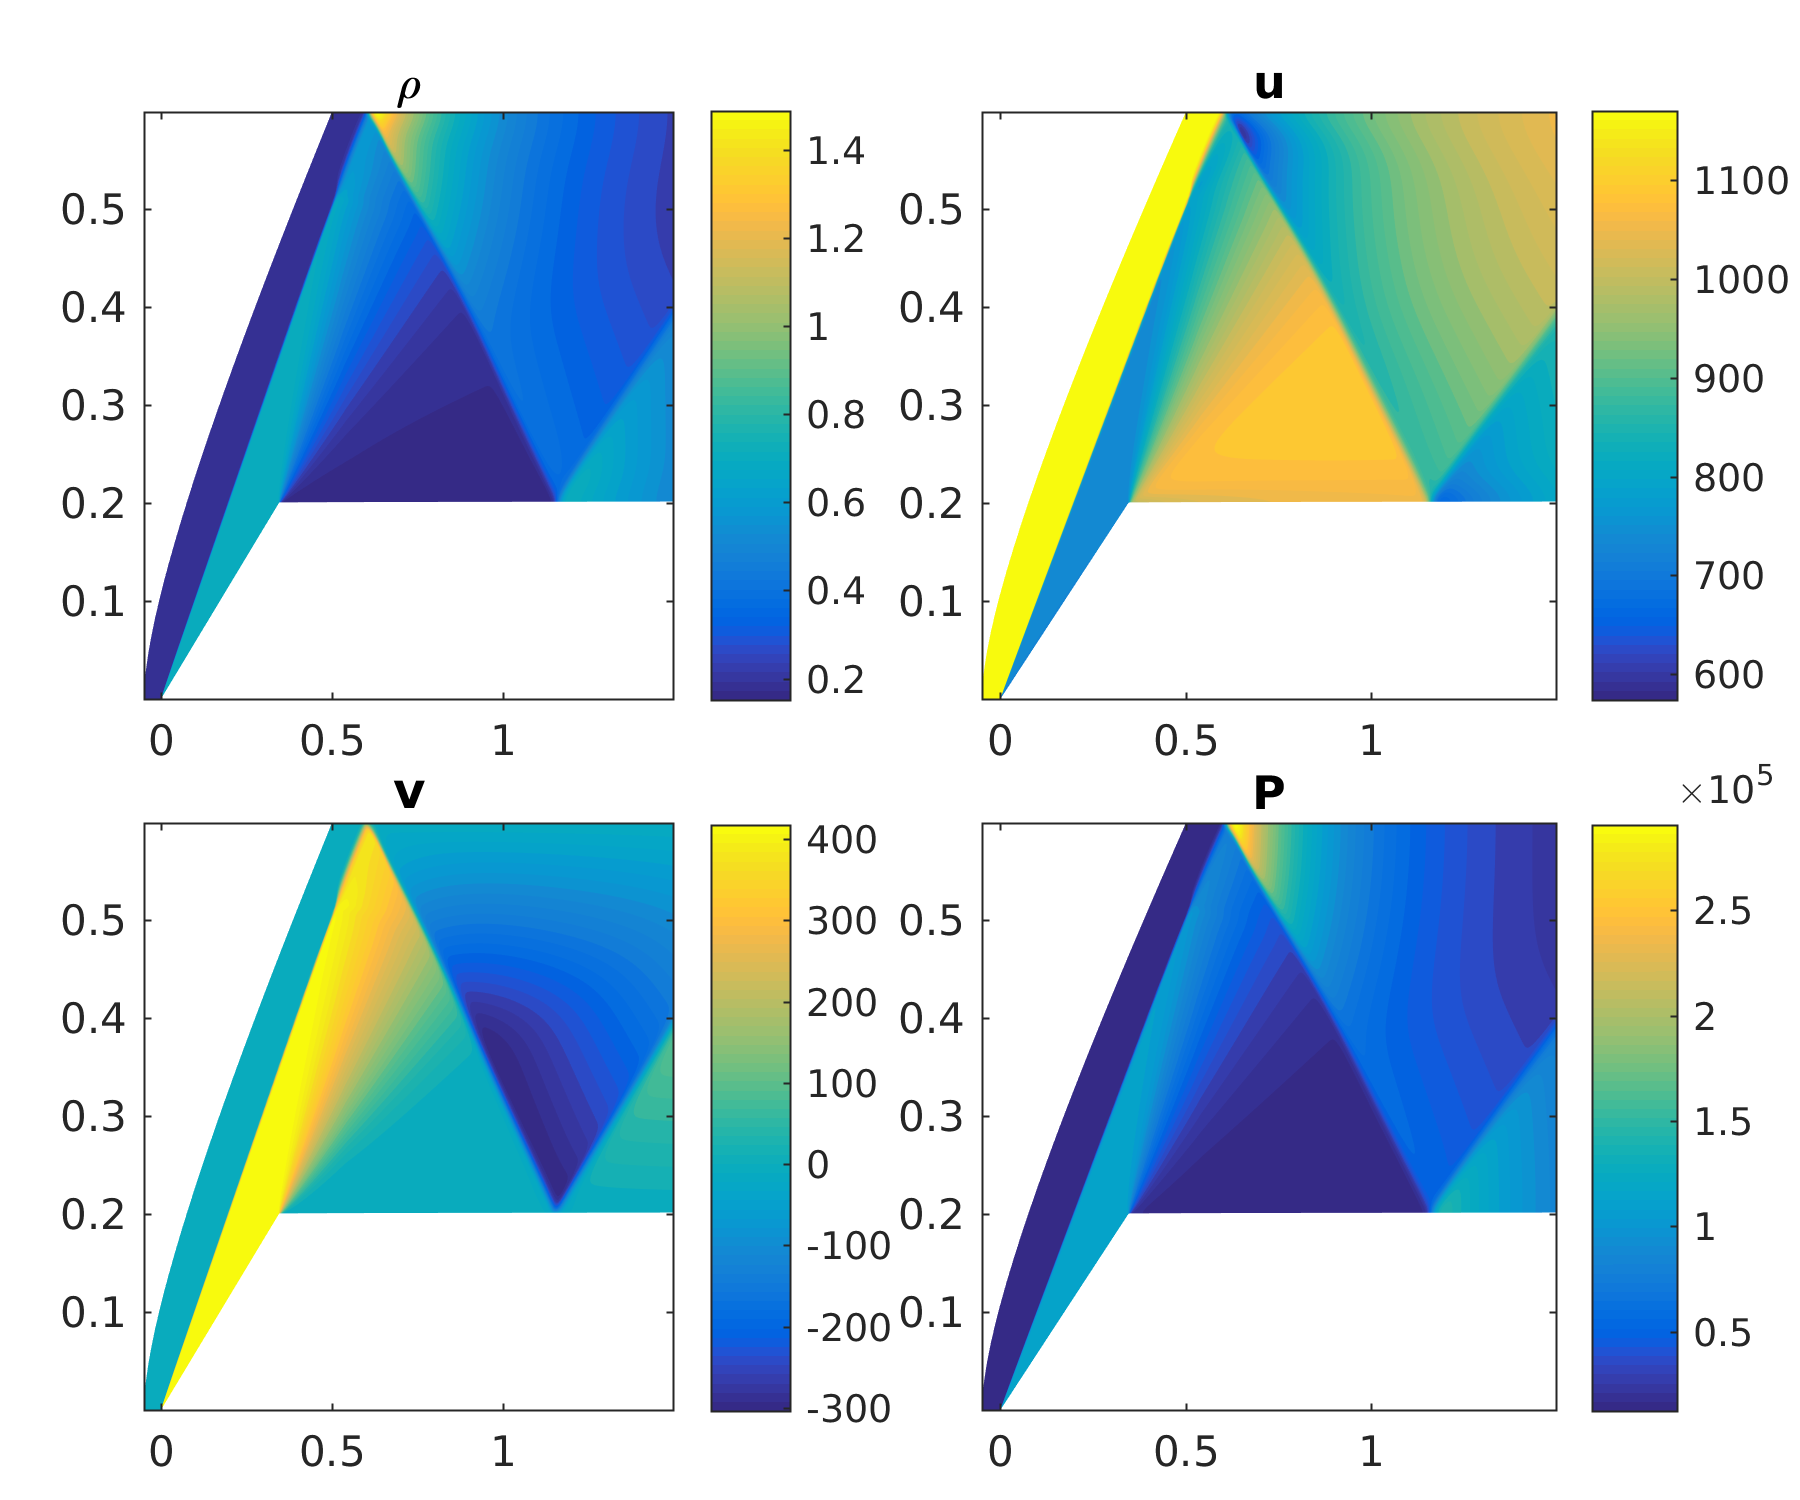
\includegraphics[width=1.0\linewidth]{fig/Inlet_mesh4_Soln}
    \centering
  \end{figure}
  \endminipage\hfill
  \endminipage
\end{frame}


\section{New Equation System \& Modeling Capabilities}

\begin{frame}[t]{Discretization $-$ 1}
 
 \vspace{-0.55cm}
  \begin{figure}[!htbp]
   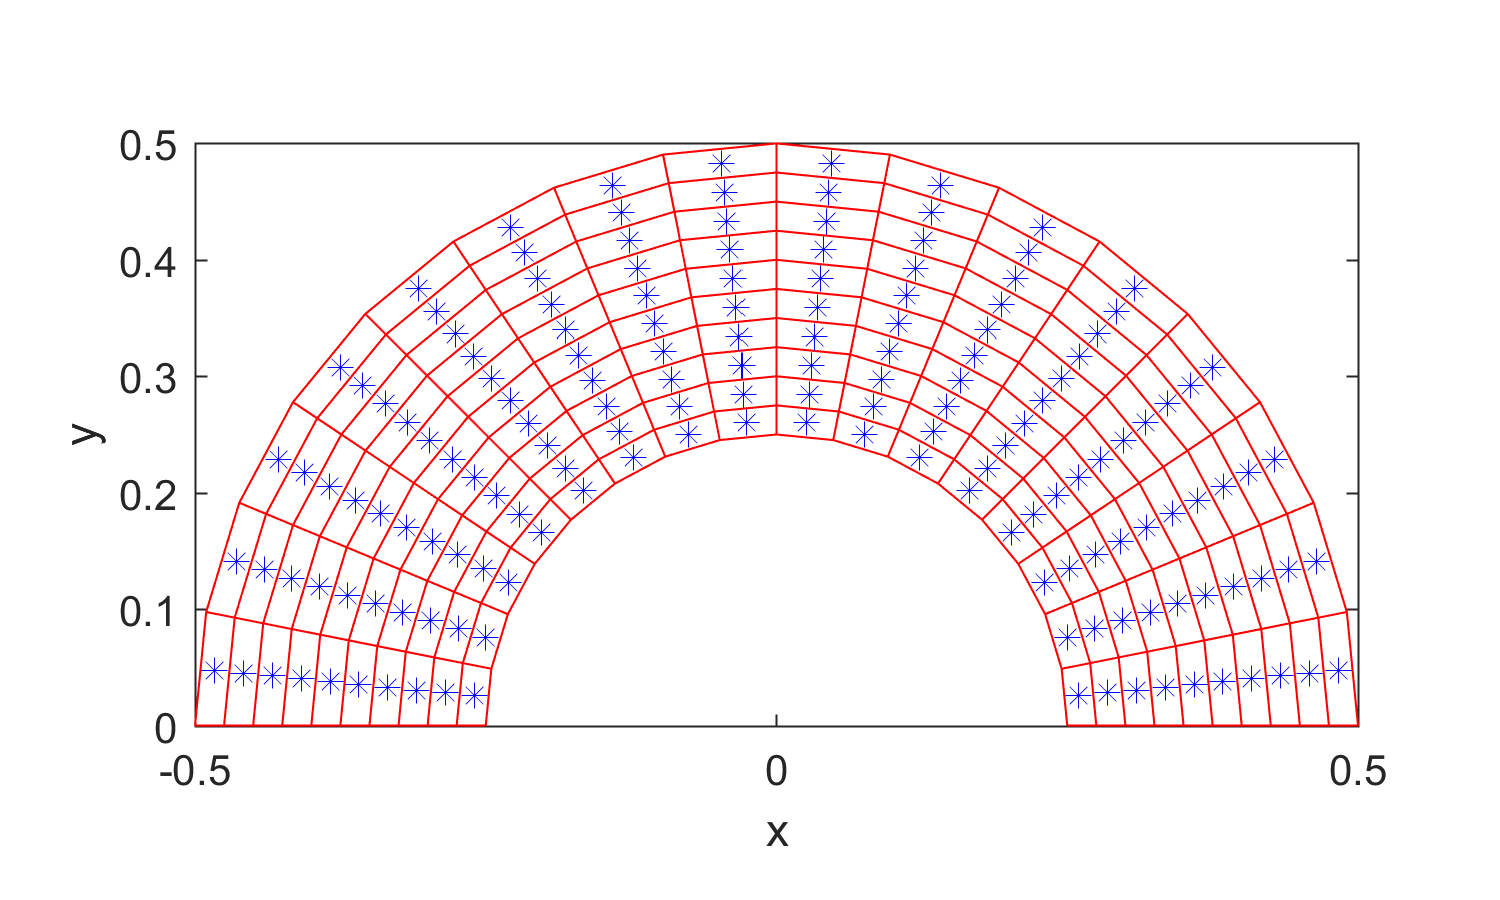
\includegraphics[width=0.85\linewidth]{../fig/16x10mesh}
   \centering
 \end{figure}

 \vspace{-0.5cm}
  \begin{itemize}
    \item Domain is discretized into cells which have constant averaged values
    \item BC: Left and Right are periodic, Top and Bottom are perfectly conducting walls.
  \end{itemize}

\end{frame}


\begin{frame}[t]{Equations}
  \minipage{\textwidth}
    \minipage{0.48\textwidth}
    \textbf{Euler Equations $\rightarrow$ MHD}
      \begin{align*}
        \pfrac{\rho}{t} + \nabla \cdot \left[\rho \mathbf{u}\right] &= 0 \\
        \pfrac{\rho \mathbf{u}}{t} + \nabla \cdot \left[\rho \mathbf{u}\mathbf{u}^T + \mathbb{I}P\right] = 0 \\
        \pfrac{\epsilon}{t} + \nabla \cdot \left[\left(\epsilon + P \right)\mathbf{u}\right] &= 0 \\
        \epsilon = \epsilon_{internal} + \frac{1}{2}\rho|\mathbf{u}|^2 &\\
        P = \rho \epsilon_{internal} (\gamma - 1) &
      \end{align*}
    \endminipage\hfill
    \minipage{0.48\textwidth}
      \begin{align*}
        \pfrac{\rho}{t} + \nabla \cdot \left[\rho \mathbf{u}\right] &= 0 \\
        \pfrac{\rho \mathbf{u}}{t} + \nabla \cdot \left[\rho \mathbf{u}\mathbf{u}^T - \mathbf{b}\mathbf{b}^T + \mathbb{I}\left(P + \frac{1}{2}|\mathbf{b}|^2\right)\right] &= 0 \\
        \pfrac{\epsilon}{t} + \nabla \cdot \left[\left(\epsilon + P + \frac{1}{2}|\mathbf{b}|^2\right)\mathbf{u}- \mathbf{b}\cdot\mathbf{u}\mathbf{b}\right] &= 0 \\
        \pfrac{\mathbf{b}}{t} + \nabla\cdot\left[\mathbf{u}\mathbf{b}^T-\mathbf{b}\mathbf{u}^T\right] &= 0\\
        \epsilon = \epsilon_{internal} + \frac{1}{2}\rho|\mathbf{u}|^2 + \frac{1}{2}|\mathbf{b}|^2 
      \end{align*}
    \endminipage\hfill
  \endminipage
  \begin{equation*}
    \text{In short hand notation:}\;\pfrac{\mathbf{Q}}{t} + \nabla \cdot \rttensor{T} = 0, \; \mathbf{Q} = [\rho,\;\rho \mathbf{u},\; \epsilon,\;\mathbf{b}]^T, \; \&\; \rttensor{T} = [\cdots]^T
  \end{equation*}
\end{frame}

\begin{frame}[t]{Finite Volume Method}
  \textbf{2D Cartesian Flux Form}: $\pfrac{\mathbf{Q}}{t} + \pfrac{\mathbf{F}}{x} + \pfrac{\mathbf{G}}{y} = \mathbf{S}$ 

\begin{equation*}
  \oiiint \pfrac{\mathbf{Q}}{t} dV + \oiint \mathbf F dA_{\hat{x}}  + \oiint \mathbf G dA_{\hat{y}} - \oiiint \mathbf{S} dV= 0
\end{equation*}

  \begin{itemize}
    \item  $\oiiint \pfrac{\mathbf{Q}}{t} dV$ $-$ Evolved using 4th Order low storage Runge-Kutta
    \item  $\oiint \mathbf F dA_{\hat{x}} \& \oiint \mathbf G dA_{\hat{y}}$ $-$ Computed from $\rttensor{T}$, but what $\mathbf{Q}$ should be used?
      \begin{itemize}
        \item Need to reconstruct a $\mathbf{Q}$ on the interface (Riemann problem $\mathbf{Q_L}\mathbf{Q_R}\rightarrow\mathbf{Q}$). The Harten-Lax-Leer ARS is used which uses max and min eigenvalues.
        \item What $\mathbf{Q_L}\&\mathbf{Q_R}$ should be used? The second order Monotone Upwinding scheme for Scalar Conservation Laws (MUSCL) is used to reconstruct the $\mathbf{Q_L}\&\mathbf{Q_R}$ states.
      \end{itemize}
    \item $\oiiint \mathbf{S} dV$ $-$ gravitational source term added to the momentum and energy equation.
  \end{itemize}
%\[
%  \pfrac{}{t}
%  \begin{bmatrix}
%    \rho  \\
%    \rho u  \\
%    \rho v \\
%    \rho w \\
%    \epsilon\\
%    b_x \\
%    b_y \\
%    b_z 
%  \end{bmatrix}
%  \;+\;\pfrac{}{x}
%  \begin{bmatrix}
%    \rho u  \\
%    \rho u^2 + P + \frac{1}{2}|\mathbf{b}|^2 - b_x^2\\
%    \rho u v - b_x b_y \\
%    \rho u w - b_x b_z \\
%    \left(\epsilon+ P + \frac{1}{2}|\mathbf{b}|^2 \right) u - b_x \mathbf{u}\cdot\mathbf{b}\\
%    0 \\
%    b_y u - b_x v \\
%    b_z u - b_x w 
%  \end{bmatrix}
%  \;+\;\pfrac{}{y}
%  \begin{bmatrix}
%    \rho v  \\
%    \rho v u - b_y b_x\\
%    \rho v^2 + P + \frac{1}{2}|\mathbf{b}|^2 - b_y^2\\
%    \rho v w - b_y b_z \\
%    \left(\epsilon+ P + \frac{1}{2}|\mathbf{b}|^2  \right) v - b_y\mathbf{u}\cdot\mathbf{b}\\
%    b_x v - b_y u \\
%    0 \\
%    b_z v - b_y w 
%  \end{bmatrix}
%  =0
%\]
\end{frame}


\begin{frame}[fragile]{Finite Volume Method - 2}
\lstset{language=C++,
                keywordstyle=\color{blue},
                stringstyle=\color{red},
                commentstyle=\color{green},
                morecomment=[l][\color{magenta}]{\#}}
\begin{lstlisting}
  ...
  mesh read
  initialize
  ...
  while(t < tend){
    for(int k = 0; k < 4; k++){
      setBC
      sourceTerm  (kernel eligible)
      MUSCL LR & BT (kernel eligible)
      2dflux F & G (kernel eligible)
      residual (kernel eligible)
      rungeKutta (kernel eligible)
    }
  }
  return 0;
}
\end{lstlisting}
\end{frame}

\begin{frame}[t]{Storage \& Indexing}
  \minipage{\textwidth}
  \minipage{0.35\textwidth}
  \textbf{Notes on storage}
  \begin{itemize}
    \item Row major storage used 
    \item 3 ghost layers shown
    \item $\mathbf{Q}$ is stored as $\rho_0, u_0, v_0, \dots, \rho_1, u_1, v_1, \dots$
    \item Eigen Matrix map double array
  \end{itemize}


  \endminipage\hfill
  \minipage{0.62\textwidth}
 \begin{figure}[!htbp]
   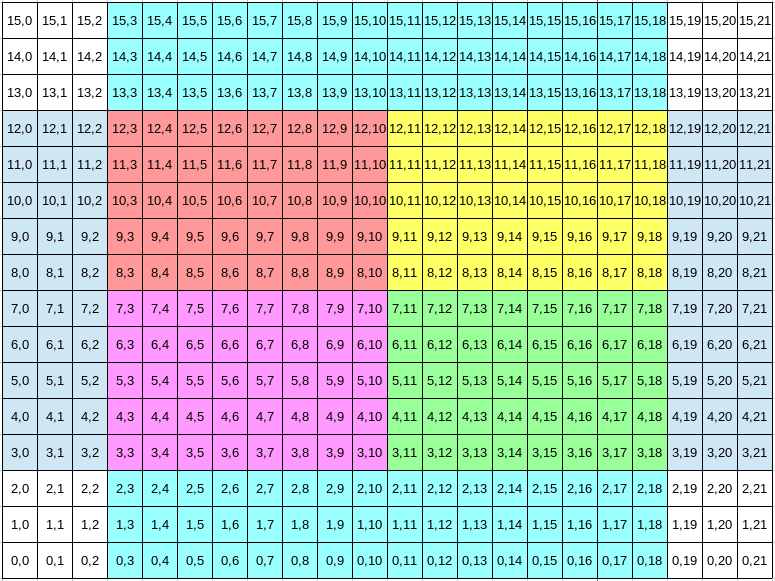
\includegraphics[width=1.0\linewidth]{../fig/16x10compDomain}
   \centering
 \end{figure}
  \endminipage\hfill
  \endminipage

\end{frame}


\section{Parallel \& GPU}

\begin{frame}[t, label=current]{Revisit Direct Drive/RT}
  \minipage{\textwidth}
  \minipage{0.57\textwidth}
  \begin{figure}[!htbp]
   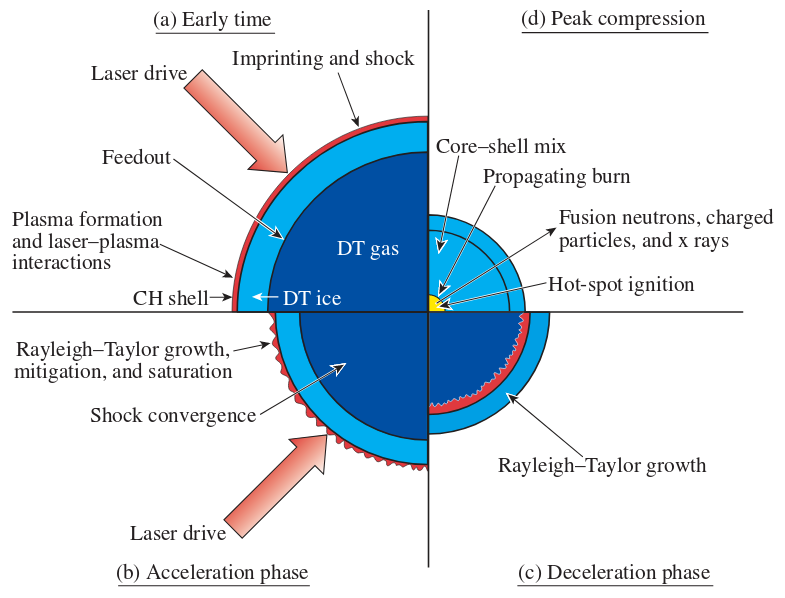
\includegraphics[width=1.0\linewidth]{../fig/DDfusion}
   \centering
  \end{figure}

  \endminipage\hfill
  \minipage{0.42\textwidth}
  \begin{itemize}
    \item Heavy fluid 
    \item Light fluid
    \item Gravity 
    \item Stabilizing Magnetic fields
  \end{itemize}
  \endminipage\hfill
  \endminipage
  \vspace{-0.5cm}
 \footnote{\cite{craxton2015}}
\end{frame}


\begin{frame}[t]{Parallel - Base}
  \textbf{Density growth at t=0.12891, 560x480}
  % took 3 mins
 \begin{figure}[!htbp]
   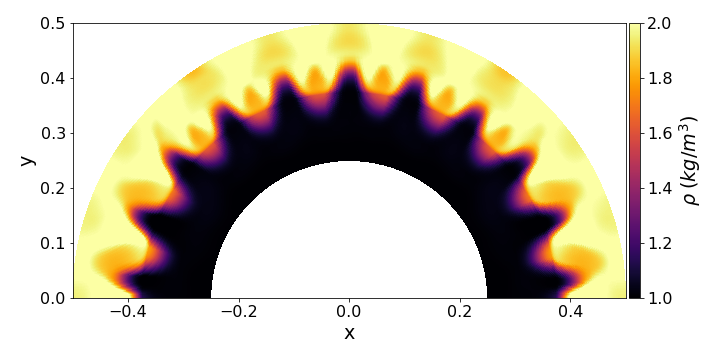
\includegraphics[width=0.85\linewidth]{fig/560x480cpuBase}
   \centering
 \end{figure}
\end{frame}



\begin{frame}[t]{Parallel - Effect of g}
  \textbf{Density growth at t=0.12891 with 5xg, 560x480}
  % took 3 mins
 \begin{figure}[!htbp]
   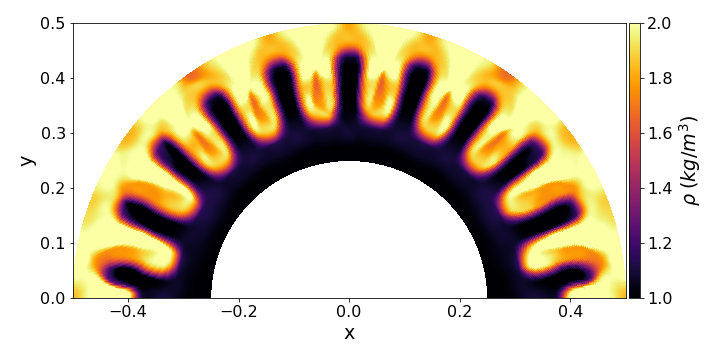
\includegraphics[width=0.85\linewidth]{fig/560x480cpu}
   \centering
 \end{figure}
\end{frame}

\begin{frame}[t]{Parallel - Effect of Bt}
  \textbf{Density growth at t=0.12891 with 5xg and 10xBt, 560x480}
  % took 3 mins
 \begin{figure}[!htbp]
   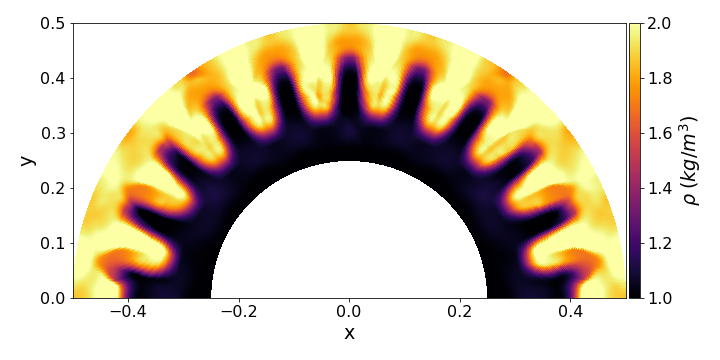
\includegraphics[width=0.85\linewidth]{fig/560x480cpuBx}
   \centering
 \end{figure}
\end{frame}

\begin{frame}[t]{Parallel - Effect of Bt}
  \textbf{Density growth at t=0.12891 with 5xg and 50xBt, 560x480}
  % took 3 mins
 \begin{figure}[!htbp]
   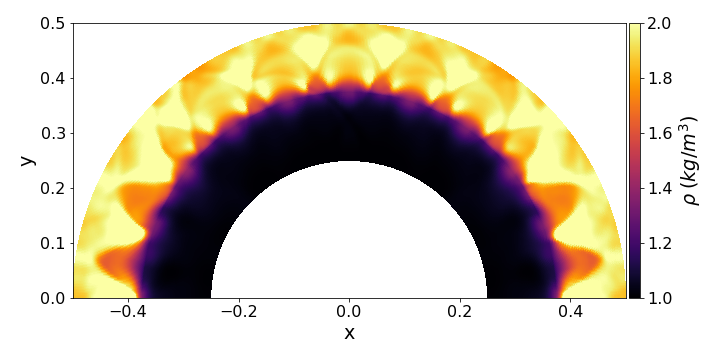
\includegraphics[width=0.85\linewidth]{fig/560x480cpuBx5}
   \centering
 \end{figure}
\end{frame}

\begin{frame}[t]{Parallel - Effect of Bt}
  \textbf{Bx growth at t=0.12891 with 5xg and 50xBt, 560x480}
  % took 3 mins
 \begin{figure}[!htbp]
   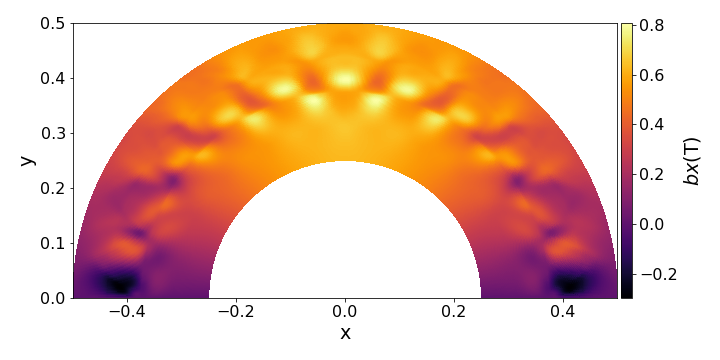
\includegraphics[width=0.85\linewidth]{fig/560x480cpuBx5_bx}
   \centering
 \end{figure}
\end{frame}



\begin{frame}[t]{Converting to GPU}
  \textbf{Converting CPU $\rightarrow$ GPU Challenges}
  \begin{itemize}
    \item CPU heavily utilized the matrix library Eigen challenges are met in the indexing ($Q[rhoid](i,j)$ vs $Q[(i*nic+j)*NEQ+rhoid]$)
    \item Host is used for mesh construction, $\mathbf{Q}$ initialization, and mpi set bc
    \item Geometry (normal vecs, areas, volumes) and initialized $\mathbf{Q}$ are loaded onto device
    \item On device: sourceTerm, MUSCL LR BT, 2dFlux F G, residual, and rungekutta
    \item $\mathbf{Q}$ is copied back to host for halo exchange
  \end{itemize}

  \textbf{Note}
  \begin{itemize}
    \item Currently does not run successfully encountering issues (develops nans)
    \item But characteristics on performance can be measured for the first few frames. 
  \end{itemize}
\end{frame}




\begin{frame}[t]{Roofline Modeling}
  %\vspace{-0.5cm}
  \minipage{\textwidth}
  \minipage{0.82\textwidth}
  \begin{figure}[!htbp]
   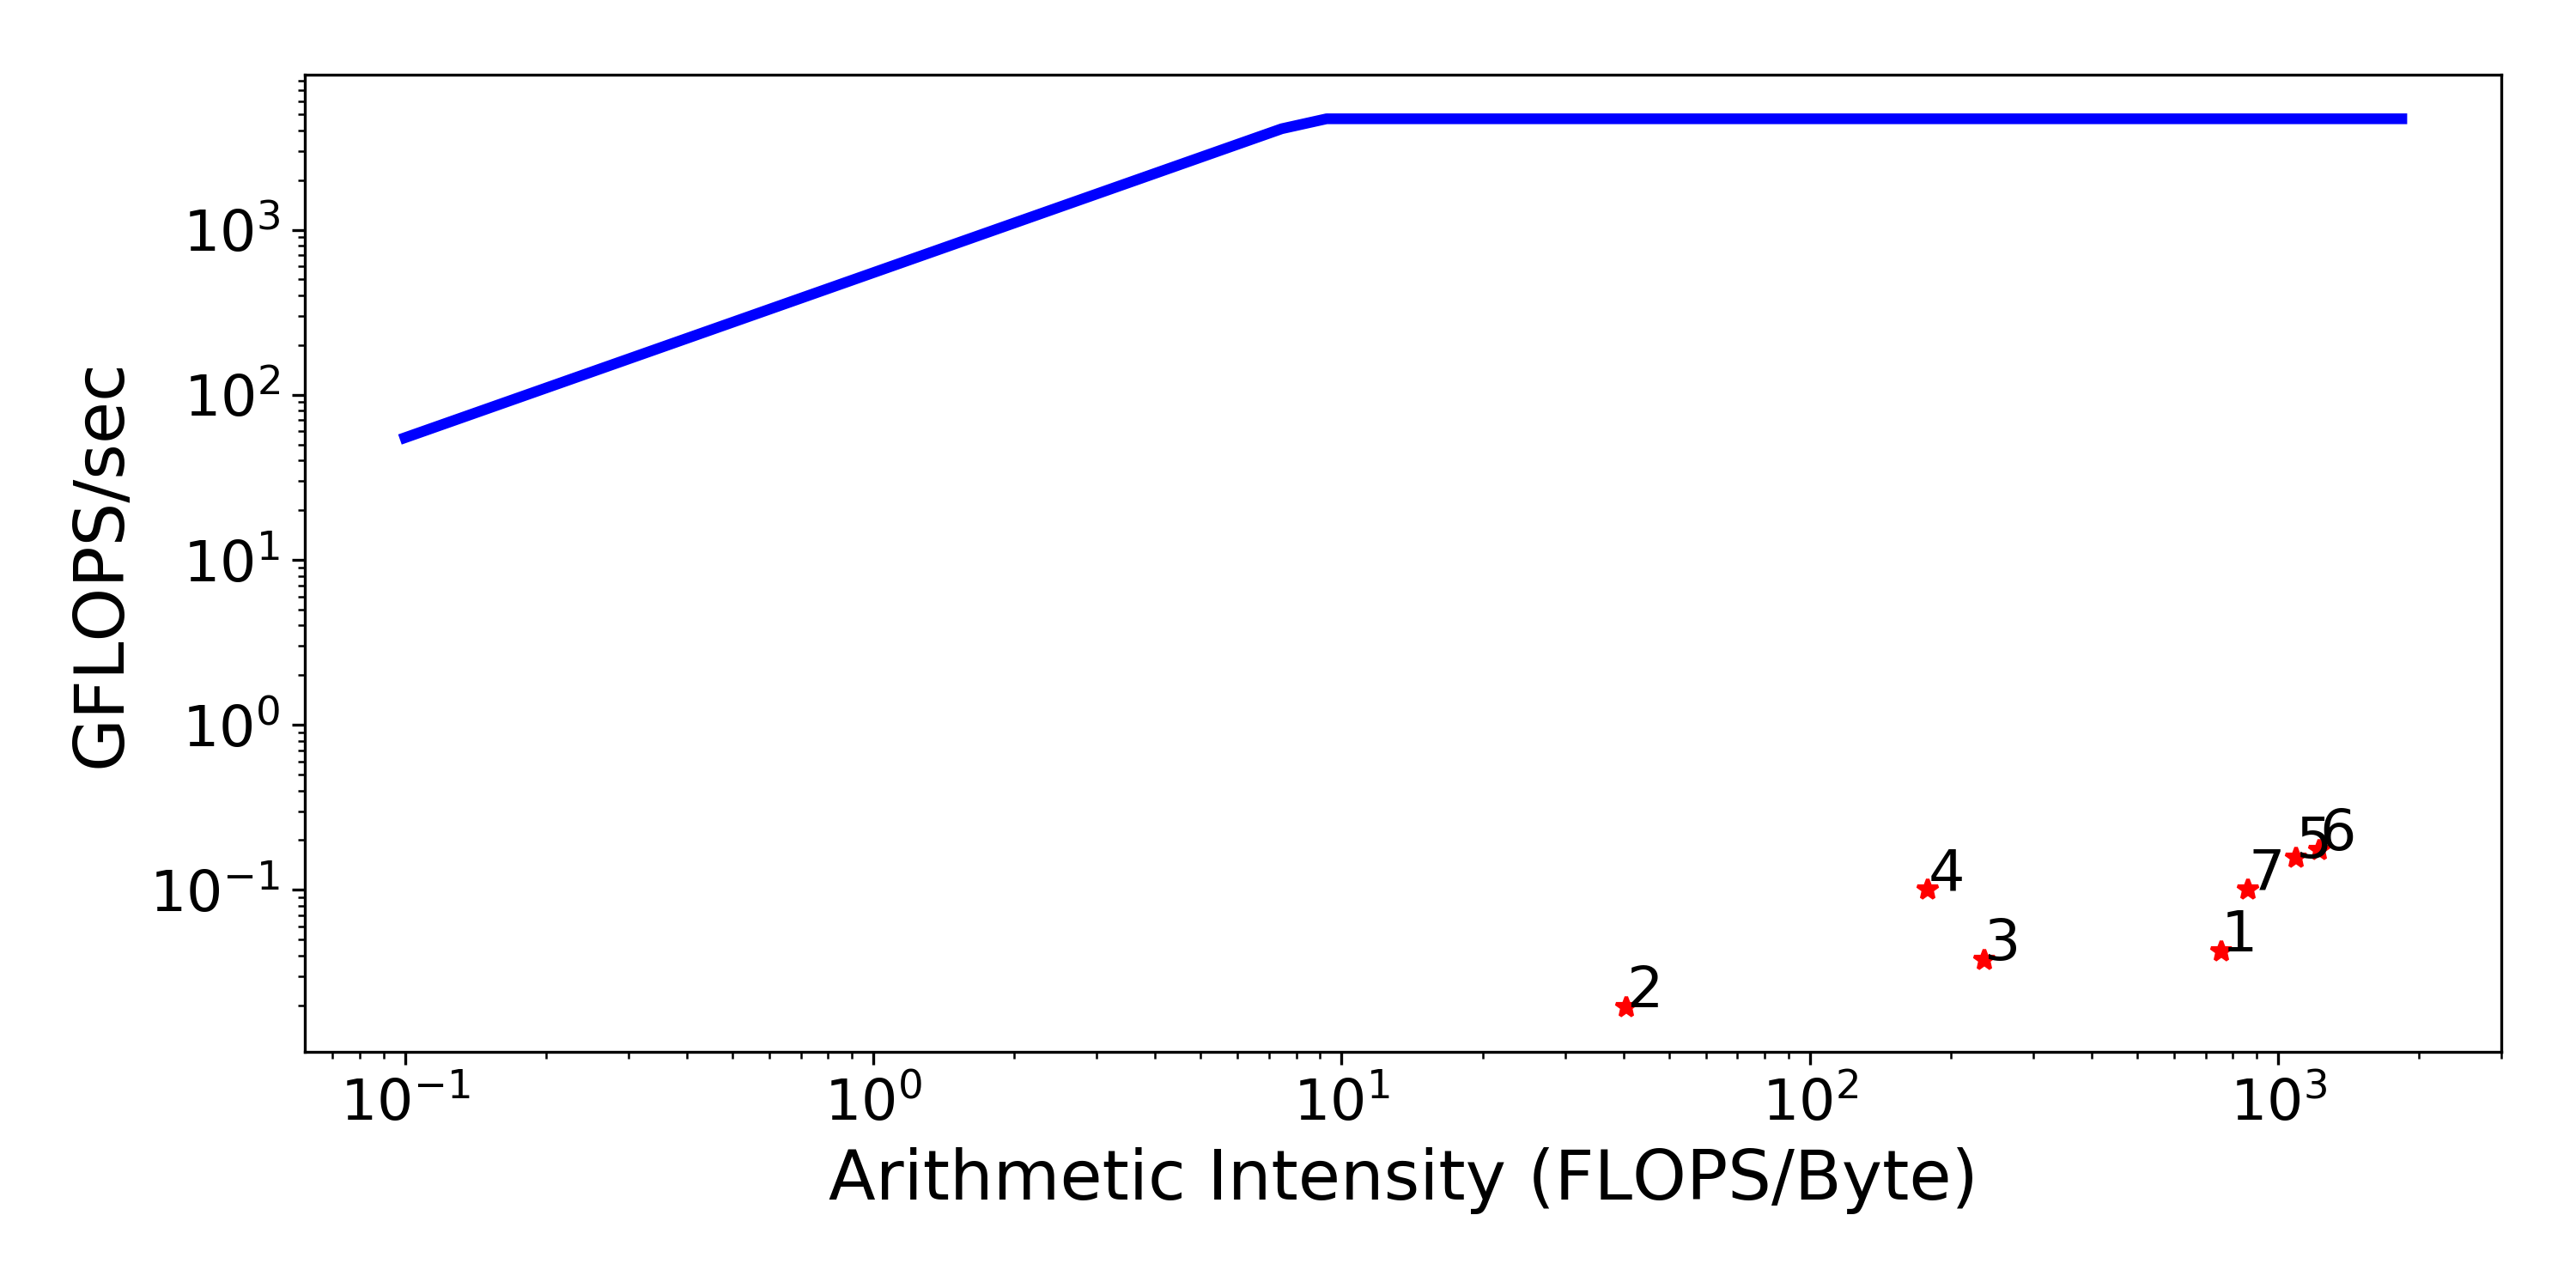
\includegraphics[width=1.0\linewidth]{fig/rooflinemodeling}
   \centering
  \end{figure}

  \endminipage\hfill
  \minipage{0.17\textwidth}
    1 source term \\
    2 residual\\
    3 runge kutta\\
    4 MUSCL LR\\
    5 2dFlux F\\
    6 2dFlux G\\
    7 MUSCL BT
  \endminipage\hfill
  \endminipage


  \vspace{0.5cm}
  %\tiny{I tried}
\end{frame}

\begin{frame}[t,fragile]{Questions? \& Plan}
  \textbf{Next Steps}
  \begin{itemize}
    \item Check initialization for issue with interface 
    \item Fix the periodic boundary conditions
    \item Verification and Validation study on the code
    \item Further debug OCCA kernels
    \item Optimize kernels
    \item Begin mpi with multiple gpu test case
  \end{itemize}
\end{frame}

\backupbegin

\begin{frame}[t]{Serial}
  \textbf{Density growth at n = 1000, 360x300}
 \begin{figure}[!htbp]
   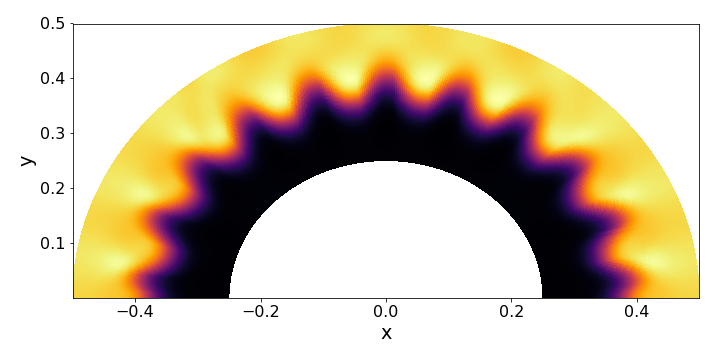
\includegraphics[width=0.85\linewidth]{fig/360x300serial}
   \centering
 \end{figure}
\end{frame}

\begin{frame}[t]{Parallel}
  \textbf{Density growth at n = 1000, 360x300}
 \begin{figure}[!htbp]
   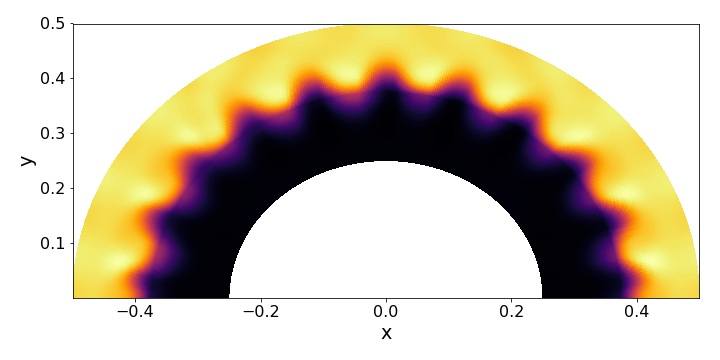
\includegraphics[width=0.85\linewidth]{fig/360x300parr2}
   \centering
 \end{figure}
\end{frame}




\begin{frame}[t]{Parallel $-$ 3}
 \textbf{Bugged}
 \begin{figure}[!htbp]
   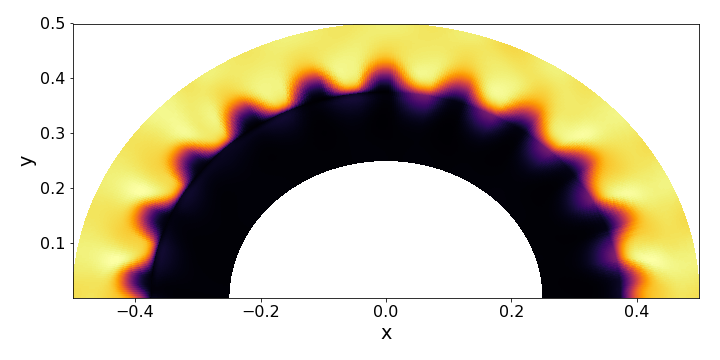
\includegraphics[width=0.85\linewidth]{fig/360x300parr}
   \centering
 \end{figure}
\end{frame}

\begin{frame}[t,fragile]{References}

  \tiny
  \bibliographystyle{plainnat}
  \bibliography{../reference}
\end{frame}





\backupend






